\documentclass[lineno,authoryear]{FLO_v1}%

%%%% Packages
\usepackage{graphicx}
\usepackage{upgreek}
\usepackage{multicol,multirow}
\usepackage{amsmath,amssymb,amsfonts}
\usepackage{mathrsfs}
\usepackage{amsthm}
\usepackage[figuresright]{rotating}
\usepackage{appendix}
\usepackage[authoryear]{natbib}
\usepackage{ifpdf}
\usepackage[T1]{fontenc}
\usepackage{newtxtext}
\usepackage{newtxmath}
\usepackage{textcomp}
\usepackage{xcolor}

%\renewcommand\theequation{\arabic{equation}}
%\setcounter{equation}{0}

\usepackage[colorlinks,allcolors=blue]{hyperref}
\definecolor{jourcolor}{cmyk}{1,0.57,0.01,0.38}
\hypersetup{
    colorlinks,%
    citecolor=jourcolor,%
    filecolor=jourcolor,%
    linkcolor=jourcolor,%
    urlcolor=jourcolor
}
\newtheorem{theorem}{Theorem}[section]
\newtheorem{lemma}[theorem]{Lemma}
\theoremstyle{definition}
\newtheorem{remark}[theorem]{Remark}
\newtheorem{example}[theorem]{Example}
%\numberwithin{equation}{section}

\articletype{RESEARCH ARTICLE}

\DOI{10.1017/flo.2021.1}

\Year{2021}

\Vol{1}

\Price{}

%\firstpage{1}

\art-id{FLO2000049}

%\citearticle{Bharadwaj, R., \& Santiago, J. G.}

%\Enumber{E1}%Please cbange the value of Enumber here

\begin{document}

\title[On the unsteady dynamics of  a flexible canopy at low Cauchy numbers]{On the unsteady dynamics of  a flexible canopy at low Cauchy numbers}

\author[L. Hong, R.C. Houseago, D. Parsons, J.L. Best and L.P. Chamorro]{Liu Hong$^{1}$, Robert C. Houseago$^{2}$, Daniel Parsons$^{2}$, James L. Best$^{3,4,5}$ and Leonardo P. Chamorro$^{1,3,5,6\ast}${{\href{https://orcid.org/0000-0001-8652-5411}{}}}}

%\author[2]{Juan G. Santiago}

%\authormark{Rajiv Bharadwaj and Juan G. Santiago}

\address[1]{Mechanical Science and Engineering, University of Illinois, Urbana, IL 61801, USA}
\address[2]{School of Environmental Sciences, University of Hull, HU6 7RX, UK}
\address[3]{Geology, University of Illinois, Urbana, IL 61801, USA.}
\address[4]{Geography and GIS, University of Illinois, Urbana, IL 61801, USA.}
\address[5]{Civil and Environmental Engineering, University of Illinois, Urbana, IL  61801, USA.}
\address[6]{Aerospace Engineering, University of Illinois, Urbana, IL 61801, USA.}
 


\corres{*}{Corresponding author. E-mail:
\emaillink{lpchamo@illinois.edu}}

\keywords{Electrokinetic systems; Electrophoresis}

\date{\textbf{Received:} XX 2020; \textbf{Revised:} XX XX 2020; \textbf{Accepted:} XX XX 2020}

\abstract{The unsteady dynamics of a fully-submerged canopy with relatively low flexibility and the induced turbulence were explored experimentally under small Cauchy numbers $Ca\lesssim 10$. Complimentary inspection of the flow around similar canopy but with rigid blades was also performed to understand the distinct effect of the reduced flexibility of the canopy better. Both type of canopies were composed of prismatic structures arranged in a staggered pattern and placed within a developed boundary layer. Particle image velocimetry (PIV) and particle tracking velocimetry (PTV) were used to characterize the turbulence and the motions of the elements within the center of the flexible canopy along the span of the array. Results show a significant modulation of the reconfiguration and oscillations of the plates within the first rows on the flow dynamics. The restricted flexibility produced a downstream shift of the onset of the internal boundary layer with increasing Reynolds number. Friction at the canopy height resulted lower in the flexible structure even in the region where plates underwent negligible reconfiguration, evidencing the impact of the leading structures on the flow adjustment. The same phenomenon occurred with the vertical mixing length. The mean plate reconfiguration decreased, in general, with the distance from the leading row and became negligible past ten rows. However, the displacement intensity of the blades peaked in the fourth and fifth rows with a magnitude of the same order along the canopy.}

\maketitle

\begin{boxtext}

\textbf{\mathversion{bold}Impact Statement}

%Electrokinetic microfluidic systems have been leveraged for a wide variety of applications including sample preparation, species separation, and detection of chemical and biochemical species. One key functional aspect of such devices is field amplified sample stacking (FASS) which is used to preconcentrate species to improve the limits of detection. We demonstrate how electrophoretically transported species can exhibit shockwave and rarefaction wave phenomena. These result from a non-linear coupling between non-uniform concentration gradients and the direction of ion migration. In particular, we find ionic migration in the direction of decreasing species velocity results in self-steepening of ion gradients into a shock wave. These waves have application to efficient preconcentration of species to improve limit of detection and to species transport with minimal dispersion. Conversely, ion migration in the direction of increasing species velocity results in rarefaction waves. Importantly, experimental observations of such rarefaction waves appear qualitatively as a rapid diffusion, but in fact the dispersion rate of these waves is dominated by the non-uniform species velocity. The analyses identify key controlling parameters governing the dynamics of these waves and offers a method to enhance and suppress them.
The

\end{boxtext}

\section{Introduction}

Canopies comprising large arrays of rigid or flexible structures are ubiquitous throughout natural environments, and instrumental in a range of engineering applications. Quantifying the distinct fluid-structure interaction and changes in the structure of the flow within and around such canopies is crucial to optimize processes at various spatial scales. In nature, aquatic vegetation canopies  strongly modulate flows \citep{gambi1990flume,chen2013flow}, attenuate waves \citep{fonseca1992preliminary,paul2012wave}, and regulates the turbulence impacting sediment transport, deposition \citep{lefebvre2010influence,ortiz2013mean}, nutrient fluxes \citep{mcglathery2007eutrophication, lawson2012enhancement}, and spore dispersion within agricultural crop fields \citep{mccartney1994dispersal}. In engineering, canopies contribute to the mixing of scalars and fluxes [REF] and offer the potential for energy harvesting via, e.g., piezoelectric devices \citep{bae2014flutter}, among others.
A review of aquatic vegetation canopy flows by \citet{nepf2012flow} points out that while the frontal area modulates the mean flow, characteristics turbulent length scales are set by the stem width or diameter and spacing, and indicated the possible spatial and temporal flow variability due to canopy oscillations. Quantification of the interaction between flow and flexible canopies is a requirement in the understanding of the distinct processes over the boundary layer above the canopy. 


Flexible structures exposed to flows undergo reduced drag compared to a rigid counterpart \citep{vogel1984drag, gosselin2010drag}.  \cite{luhar2011flow} assessed the role of blade stiffness and buoyancy on blade reconfiguration, and proposed a model for drag and extent of reconfiguration, applicable to seagrass and microalgae in natural settings. Their model defines the degree of reconfiguration as a function of the dimensionless ratio of drag to stiffness restoring force (Cauchy number, $Ca$) and the ratio of the restoring force due to buoyancy and the stiffness (buoyancy parameter, $B$), defined as $Ca=\rho_f bl^{3}U^{2}/(EI)$ and $B= (\rho_f - \rho_v) gbdl^{3}/(EI)$, where  $\rho_{f}$ and $\rho_{v}$ are the fluid and blade material densities,  $b$, $d$ and $l$ are the width, thickness and length of each blade,  $U$  is the bulk incoming velocity, $E$ is the Young Modulus, and  $I$  is the second moment of inertia \citep{luhar2016wave}. In addition to the material properties, the blade geometry further alters the reconfiguration behavior \citep{albayrak2012flow}, and the unsteady dynamics \citep{jin2018flow}.

\citet{naudascher2017flow} discussed three mechanisms of flow-induced motion (FIM) of flexible elements, namely, i) an instability-induced excitation (IIE) due to a self-induced flow instability, such as wake turbulence generated by vortex shedding, including vortex-induced vibrations (VIVs), ii) an extraneously-induced excitation (EIE) caused by incoming flow fluctuations that develop independently from the plate, and iii) a motion-induced excitation (MIE) that occurs as a result of changes in the surrounding fluid forces due to the plate vibration. The motion of flexible plates can result from one process or multiple FIM processes. The frequency of VIV of a flexible structure usually corresponds to the well-known Strouhal relationship, such that the frequency of vortex shedding  $f_v= \frac{S_tU}{L}$, where  $S_t$  is the Strouhal number, and $L$ is the blade length scale, which is the diameter in cylindrical structures. \citet{jin2018instability} noted a decoupling between the frequency of the natural blade frequency and wake flow fluctuations; vortex shedding following the Strouhal relationship may occur without inducing blade motion and reasoned this was due to the dependence on blade stiffness. Characterization of such dynamics in flexible canopies is currently limited.

The presence of neighboring flexible plates may lead to distinct dynamics and flow, with such interactions being dependent on the relative spacing and alignment of the structures. \citet{kim2010constructive} found that due to vortex shedding from an upstream flag, the drag on a downstream structure either increased or decreased depending on the phase. \citet{jin2018couple} inspected two plates in tandem, and noted that the motion of the upstream plates was related to the natural blade frequency, whereas the oscillations of the downstream body depended on the structure of the flow shed from the upstream plate. This coupled effect is dependent on the separation between the blades, with the reduced coupling at increased spacing. The motions of singular and tandem blades are instrumental in understanding the flow-structure interaction in complex canopies.

The dynamics of flexible plates within a canopy may result in distinct flows. \citet{finnigan2000turbulence} presented a comprehensive review of the flow dynamics and turbulence within terrestrial plant canopies. Canopy obstruction and imposed drag cause an inflection point in the vertical profile of streamwise velocity, leading to the formation of a shear layer susceptible to Kelvin-Helmholtz (KH) instability, which may result in a mixing layer dominated by comparatively large coherent vortices \citealp{raupach1996coherent, ghisalberti2002mixing, nepf2012flow}.  \citet{okamoto2013spatial} explored the transition of a boundary layer impinging a canopy into a fully-developed mixing layer region dominated by coherent vortices further downstream. Coherent vortices can then result in canopy motion, which has been categorized depending on the extent of the motions into negligible, gently swaying, energetic coherent waving (\textit{monami}), and prone \citep{nepf2000flow}. \citet{ghisalberti2006structure} linked canopy motion to the existence of sweep and ejection events, which in turn influence the turbulence statistics and vertical mixing. \citet{ghisalberti2006structure} highlighted significant interactions between canopy motion and hydrodynamics, finding that canopy waving resulted in a substantial decrease in turbulent momentum transfer through the shear layer. The dynamics of the plates within flexible canopies and the induced coherent flow structures remain, however, not partially understood.

A large fraction of velocity measurements above and within flexible canopies have relied on single-point measurements, with somewhat limited studies capturing the spatial distribution and dynamics of the flow field. \citet[2016]{okamoto2009turbulence, okamoto2013spatial} provided an understanding of coherent flow structures and canopy motions using particle image velocimetry (PIV) combined with simultaneous particle tracking velocimetry (PTV). In particular, \citet{okamoto2009turbulence} suggested that coherent vortices are responsible for the generation of monami, which in turn modulates momentum transfer. Recent investigation \citep{okamoto2016flow} noted the initiation of monami by positive streamwise velocity perturbations associated with vortices passing the canopy top, along with a strong correlation between streamwise velocity fluctuations and canopy motion at a comparatively low frequency.
 
Very recently, \citet{o2019dynamic} employed 2D numerical simulations to illustrate that coupled interactions between the flow and canopy plate properties may be responsible for coherent monami. Their parameterizations covered a range of mass ratios and bending rigidities and enabled canopy and plate motion to be separated into four motion-based conditions, namely, static, regular waving, irregular waving, and flapping. This variability in plate dynamics was dependent on the relationship between natural blade frequency, and the mixing layer instability frequency, in addition to sheltering effects caused by surrounding plates. The similarity of mixing layer instability and blade natural frequency resulted in regular waving, whereas deviation from this resulted in temporal and spatial differences in motion (irregular waving), or a uniform defected state (static). The flapping state was characterized by the second mode natural frequency of the plates, resulting in smaller flow structures than waving canopies, clearly indicating the role of structural properties on motion dynamics.


Besides, quantification of the distinct fluid dynamics from unsteady blades with reduced motions within fully submerged, flexible canopies remains obscure. Necessary to advancing such knowledge is the assessment of the plate motions and flow properties at high temporal and spatial resolutions to uncover the distinct role of coherent motions. Here, we use a combination of PIV and PTV to quantify the turbulence and plate motions in a canopy under very low Cauchy numbers to assess the modulation of a fraction of plate motions in canopy turbulence; comparison with a rigid case will help to evaluate such modulation further.  The experimental setup is described in $\S$2, measurements and discussion are presented in $\S$3, and the main conclusions a summarized in $\S$4.


\begin{figure}
	\centerline{\includegraphics[width=0.8\textwidth]{fig1}}
	\caption{Basic schematics of the flexible (and rigid) canopy. (\textit{a}) Top and $(b)$ side views of the staggered layout. The blue, dashed line indicates the location of the streamwise wall-normal PIV plane at the center of the canopy. Tip motions of the gray structures around the center were characterized with the PTV system.  (\textit{c}) Set-up illustrating the general dimensions, the two streamwise wall-normal FOVs covering the flexible canopy.}
	\label{canopy_model}
\end{figure}


\section{Experimental Setup}\label{sec:rules_submission}

A canopy with a reduced flexibility and a rigid counterpart were placed fully submerged in a 2.5 m long,  recirculating refractive-index-matching (RIM) flume of cross section 112.5 mm $\times$ 112.5 mm.  An aqueous sodium iodide solution of density $\rho_f = 1800$ kg m$^{-3}$ and kinematic viscosity $\nu = 1.1 \times 10^{-6}$ m$^2$ s$^{-1}$ was used as working fluid. This technique allowed measurements close to the wall, ensured uniform illumination in the interrogation regions and optical access within the rigid canopy. Additional  information about RIM can be found in \citet{blois2012versatile,bai2014refractive} and \citet{hamed2017impact}.


The flexible and rigid canopies shared the same geometry characterized by prismatic blades of height  $h=37.5$ mm, width $w=6.4$ mm or $h/w\approx 5.9$, and thickness $e=2$ mm. The blades were distributed in a staggered pattern with streamwise and transverse spacing of $S_x=\Delta x/w=1.56$ and $S_y= \Delta y/w=3.125$; see basic schematic in figure \ref{canopy_model}. This resulted in a dense canopy with total frontal area per bed unit area of $\lambda_f = $ 1.2 \citep{finnigan2000turbulence}, and a frontal area per canopy volume of $a = n_sd =$ 32 m$^{-1}$. It is worth pointing out that this arrangement is similar to that studied by \citet{hamed2017impact} with rigid, heterogeneous canopies. The model canopies covered the transverse span of the flume, had a streamwise length of $\Delta x/h\approx 5$ and was placed at $\Delta x/h\approx 19$ from the inlet. There, the incoming boundary layer of $\delta=7.5$ mm induced  negligible effects on the canopy, which was placed over a 5-mm acrylic base. The flexible canopy was casted from Silicone with a Young's Modulus of $E$ = 2.05 MPa and density $\rho_m$ = 1030 kg m$^{-3}$.

The motions of the blades within two columns along the streamwise span of the flexible canopy and induced turbulence were explored under three bulk flows ($U_b$); whereas the turbulence induced by the rigid canopy was inspected under one of the flow coinciding with the flexible counterpart. Details of the corresponding Reynolds numbers $Re_H = U_{\infty}H/\nu$, the Froude numbers $Fr = U_{\infty}/\sqrt{gH}$, Cauchy numbers $Ca = \rho_f b {U_0}^2 h^3/(EI)$ \citep{luhar2016wave} and friction velocities at the canopy height $u_* = -\langle u^\prime v^\prime\rangle ^{1/2}$ \citep{poggi2004effect, nezu2008turburence, chen2013flow} are given in table \ref{input}. Here, $g$ is the acceleration of gravity, $\langle \cdot \rangle$ is the time-averaging operator, and primes denote fluctuating quantities.

 
 \begin{table}
	\begin{center}
		\def~{\hphantom{0}}
		\begin{tabular}{ccccccc}
Case & Canopy & $U_{\infty}$  & $Re_H$   &   $Fr$ & $Ca$ & $u_*$ \\[3pt]
           &  & (m s$^{-1}$)   & ($\times 10^4$) & (-) & (-) & (m s$^{-1}$) \\
			F1 & Flexible & 0.18   & 1.84 & 0.17 & 2.3 & 0.019 \\
			F2 & Flexible & 0.27   & 2.76 & 0.26 & 5.1 & 0.028 \\
			F3 & Flexible & 0.36  & 3.68 & 0.34 & 9.0 & 0.040 \\
			R ($\Leftrightarrow$F2) & Rigid   & 0.27   & 2.76 & 0.26 & 5.1 & 0.028 \\
		\end{tabular}
		\caption{Experimental cases and basic parameters. The incoming flow on the rigid canopy R1 corresponded to the flexible canopy case in F2. }
		\label{input}
	\end{center}
\end{table}

Flow statistics and structure of the turbulence for each scenario were obtained with complementary high-resolution and high-speed particle image velocimetry (PIV) systems from TSI.  Two fields of view (FOV) located in the middle of the canopy models were illuminated by a 1 mm thick laser sheet generated by a 250 mJ pulse$^{-1}$ double-pulsed laser from Quantel. Silver-coated, hollow glass spheres of diameter 14 $\mu$m and density of 1700 kg m$^{-1}$ were used as seeding. Two thousand image pairs were acquired by an 11 megapixel (4000 $\times$ 2672 pixels), 12-bit, frame straddle, CCD camera. The image pairs were processed by the recursive cross-correlation method by using the Insight 4G software from TSI. The final interrogation window was 24 $\times$ 24 pixels with 50$\%$ overlap, resulting in a vector grid spacing $\Delta x = \Delta y = 720 \mu$m.

The plates within the two central columns of the canopy were simultaneously tracked at a frequency of 150 Hz during periods of 60 s, i.e., 9000 images, for every case. A Mikrotron EoSens 4CXP MC 4082 camera at 2 MP resolution with a Nikon AF Micro-Nikkor 50 mm lens was used for the tracking. The illumination was provided by two Stanley Lithium-Ion Halogen Spotlights. The tips of each blade were carefully marked at the center to improve the motion tracking. Finally, the raw images were processed with a pixel to distance ratio of 0.08 mm pixel$^{-1}$ by the open-source OpenPTV. Detailed information on the PTV system can be found in \citet{kim2016three}. Figure \ref{schematics} illustrates the basic characteristics of the setup.




\begin{figure}
	\centering
	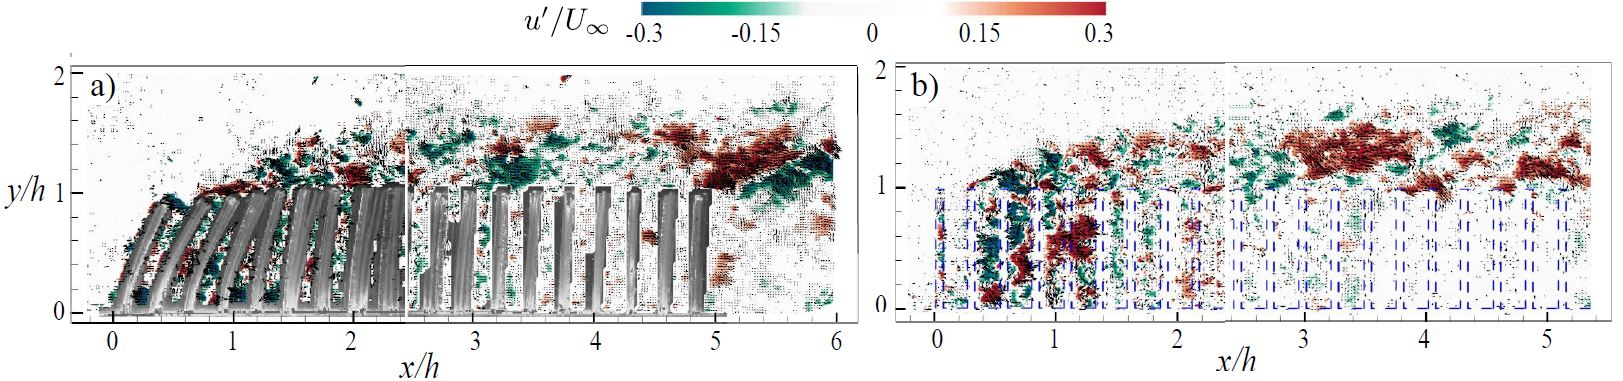
\includegraphics[width=1\linewidth]{Inst}
	\caption{Sample snapshots of the instantaneous streamwise velocity fluctuations $u'/U_{\infty}$ for the a) flexible and b) rigid canopies.}  
	\label{inst}
\end{figure} 

\section{Results}
In this section, we describe the statistics and structure of the flow around the canopy with limited blade  oscillations and explore distinct differences with the rigid counterpart. Also, we explore the features of the unsteady motions of these structures along the streamwise span of the canopy. 
The selected Cauchy numbers are such that a fraction of the blades in the first rows of the canopy undergo deformation with the rest experiencing negligible motions. This condition is possible with relatively stiff blades or relatively low flow velocity or a combination of both, which is embodied by the Cauchy number. Fundamental characterization of these type of settings is of relevance to understand unsteady loading in diverse structure arrays.


\begin{figure}
	\centering
	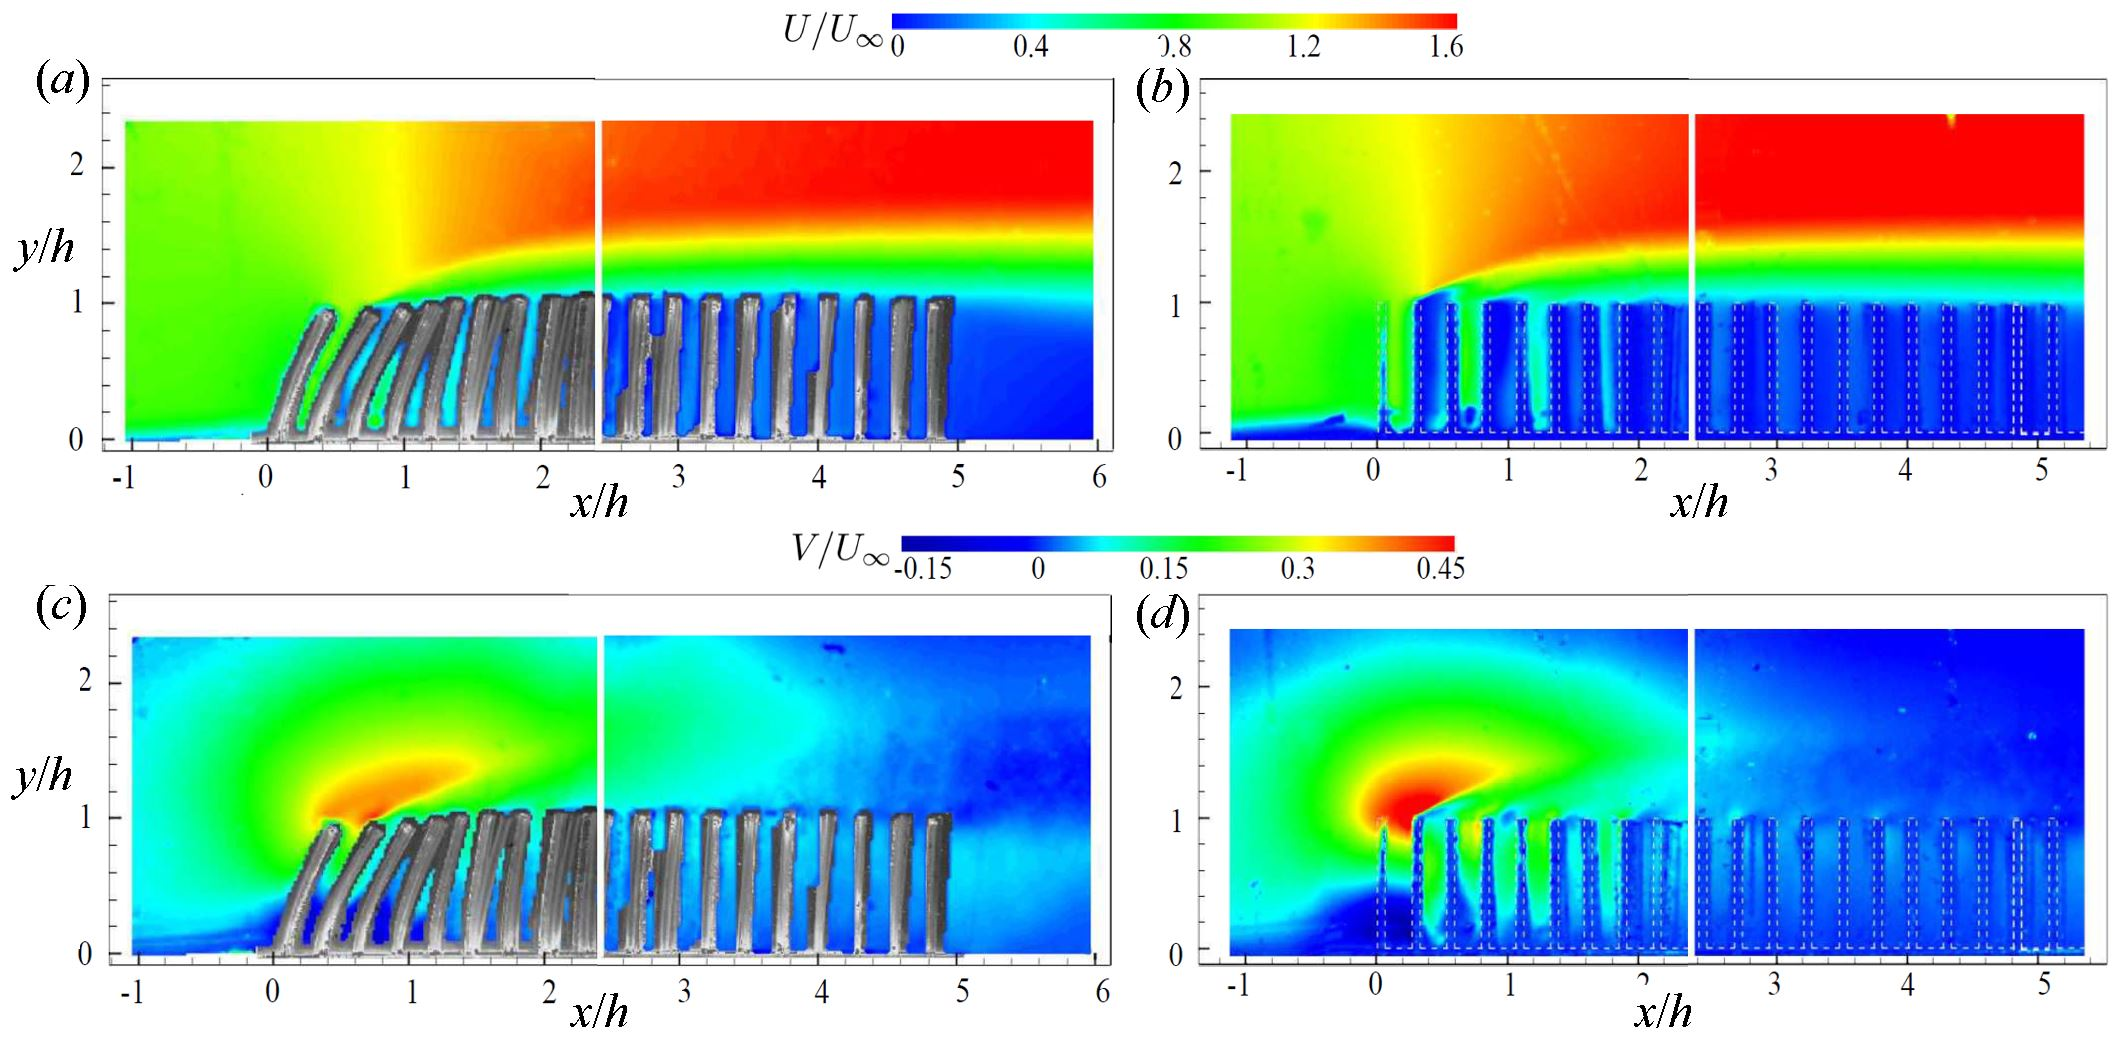
\includegraphics[width=1\linewidth]{Mean_U}
	\caption{Time-averaged distributions of the a) streamwise $U/U_{\infty}$ and b) vertical $V/U_{\infty}$ velocity components around the flexible canopy at $Re_H = 2.76\times 10^4$. c) $U/U_{\infty}$ and d) $V/U_{\infty}$ for the rigid canopy.}  
	\label{u_mean}
\end{figure}  


\subsection{On the flow field}

The relatively minor deformation and oscillations of the leading plates induced distinct changes in the flow statistics, the structure of the turbulence and exchange between the flow within and above the canopy that extended the span of the canopy. Figure \ref{inst} illustrates samples of instantaneous velocity fluctuation fields around the flexible and rigid canopies within the interrogation areas. Despite the arbitrary examples, those fields show effects that extend the canopy span and only a fraction of the plates experienced appreciable motions due to the low $Ca$. This particular canopy conceptually differs from those where all elements experience substantial flow-driven motions. 

The mean flow field reveal the impact of the plate reconfiguration and motions in the first rows, as illustrated in figure \ref{u_mean} for the case F2. It includes the streamwise $U/U_{\infty}$ and vertical $V/U_{\infty}$ velocity components; there, the rigid case is included as a reference. Despite the limited deformation of the plates in the first rows, it induces a delay in the onset of the internal boundary layer development, a reduced vertical velocity at the beginning of the canopy due to the reconfiguration and the vertical velocity over the canopy extending longer in the flexible canopy. Selected vertical profiles along and over the canopies for all the scenarios are shown in figure \ref{uprofile} to appreciate better the differences between the cases. Specifically, the downstream shift of the beginning of the internal boundary layer, $\delta_i$, with $Re$ (at $x_0/h\approx 1$, 1.3 and 1.6 for the $Ca=2.3$, 5.1 and 9.0) and the higher $\delta_i$ of the rigid case within $x\lesssim 5$. Comparison of the streamwise and vertical velocities along the canopies at the tip show the slower adjustment of the flexible canopies compared to that of the rigid case. Complementary view of the mean velocity evolution is shown with horizontal profiles 





\begin{figure}
	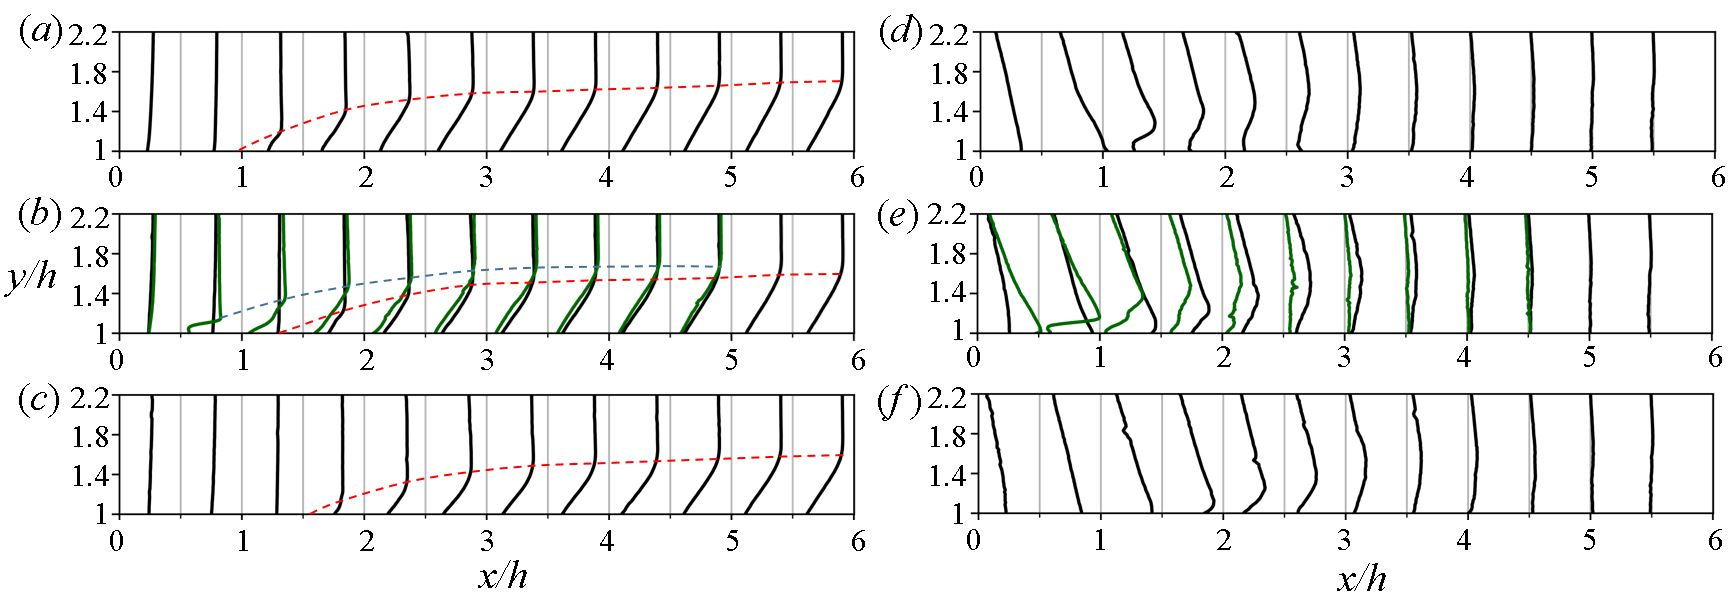
\includegraphics[width=\textwidth]{U_V_profiles}
	\caption{Vertical profiles of the streamwise velocity at $Ca=$ a) 2.3 (Case F1), b) 5.1 (cases F2), added rigid case with green curve, and c) Ca=9.0 (case F3). The red-dashed and blue-dashed lines indicate the internal boundary layer of the flexible and rigid canopies. d-f) indicate th\\
		e corresponding vertical velocity profiles.}
	\label{uprofile}
\end{figure}





\begin{figure}
	\centering
		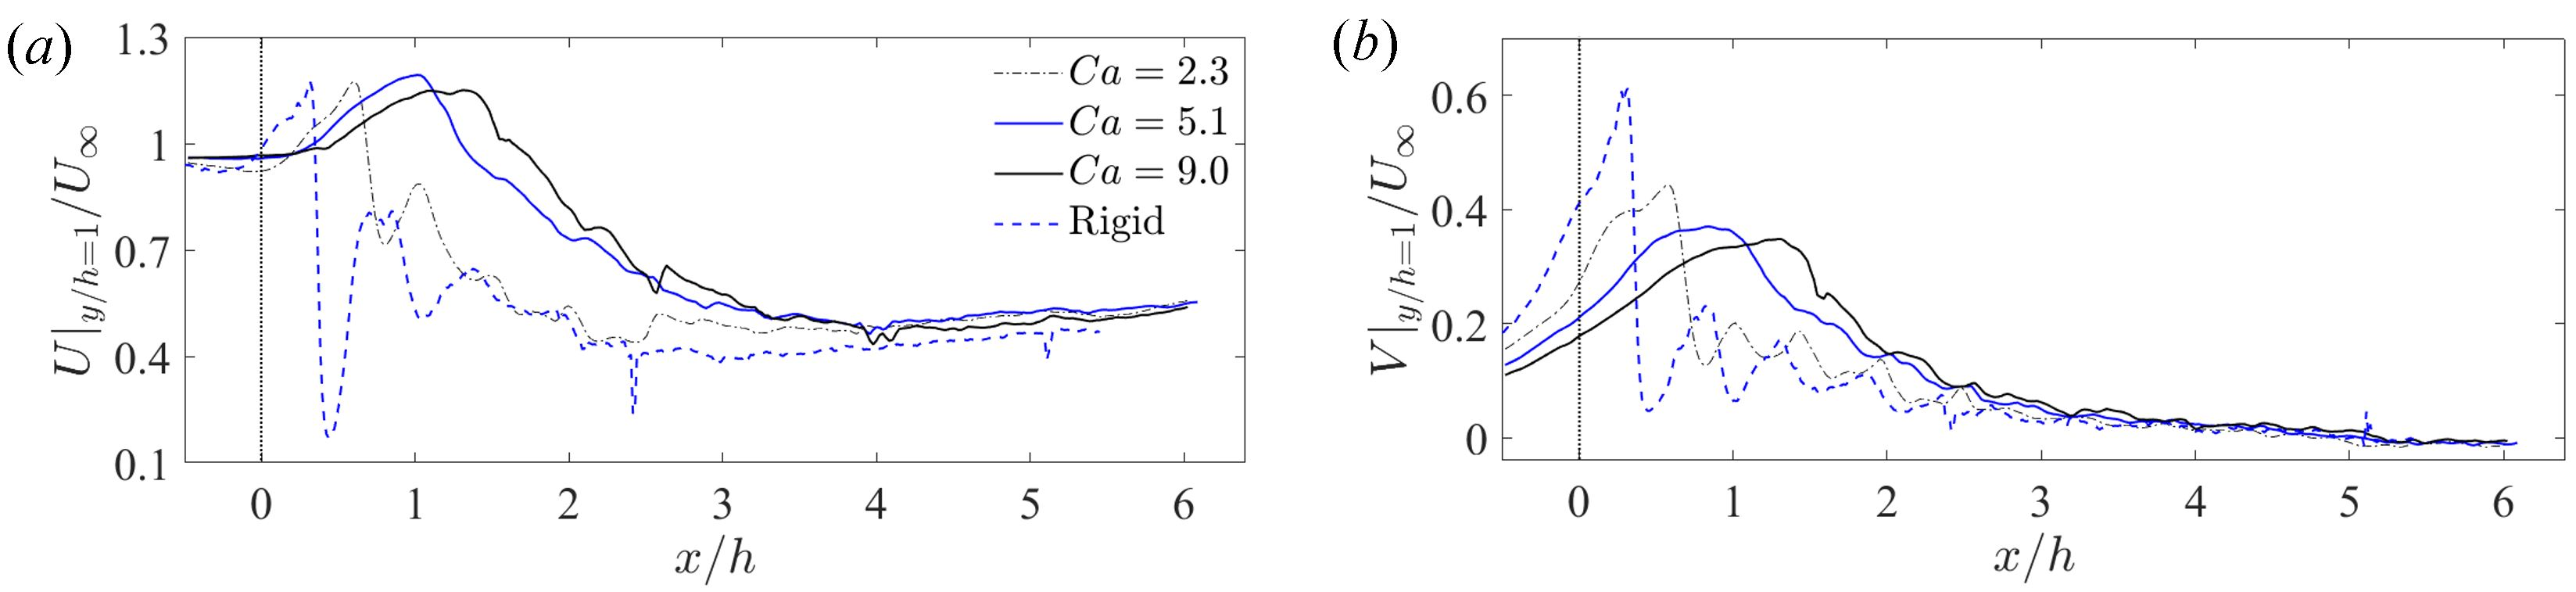
\includegraphics[width=1\linewidth]{U_V_y1}
	\caption{Figure a: time-averaged streamwise velocity profiles $U(x,y=h)/U_{\infty}$ with various incoming flow velocity; Figure b: time-averaged vertical velocity profile $V(x,y=h)/V_{\infty}$ with various incoming flow velocity.}
	\label{velocity_yh}
\end{figure}

 

 

\begin{figure}
	\centerline{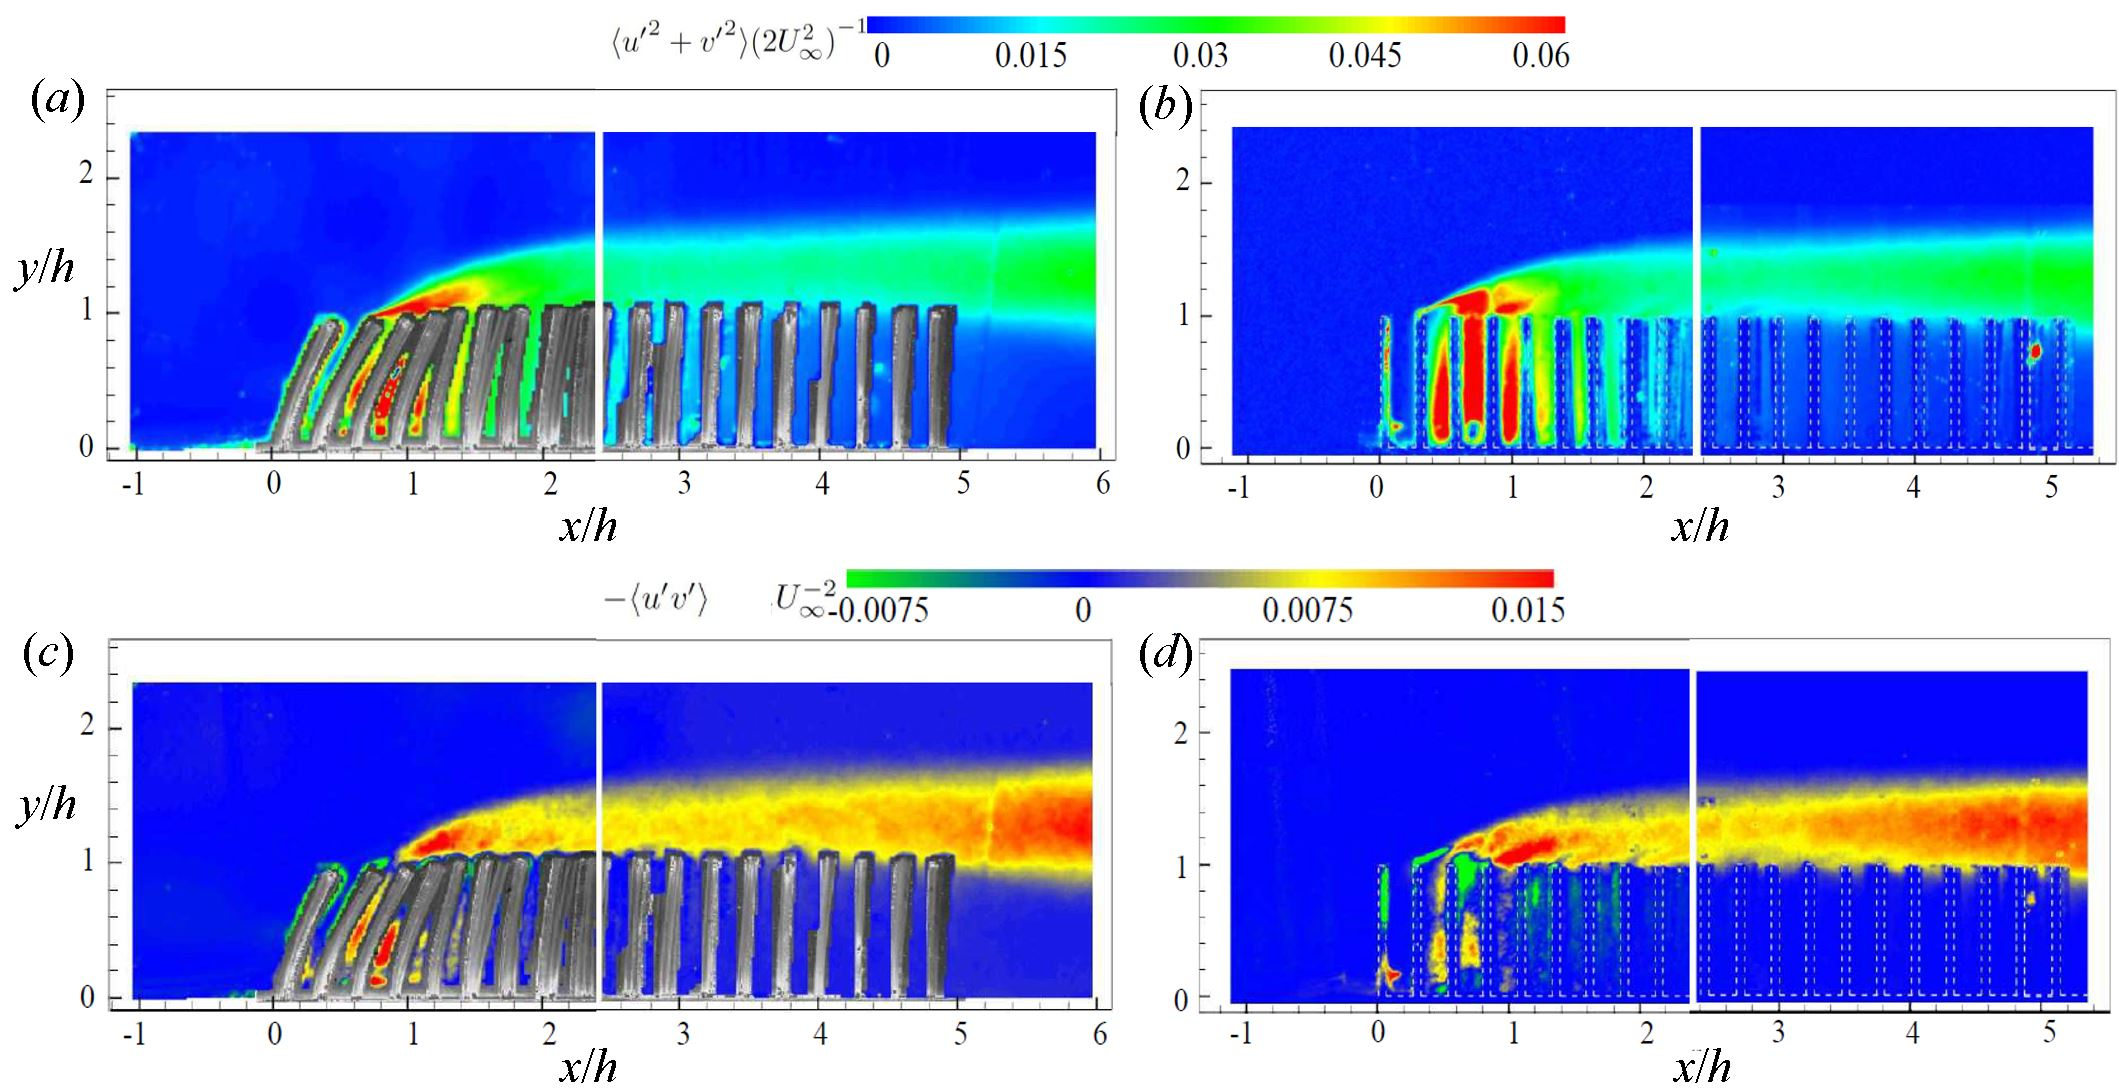
\includegraphics[width=1\textwidth]{TKE_uw}}
	\caption{In-plane turbulence kinetic energy, $TKE = \langle {u^{\prime}}^2 + {v^{\prime}}^2 \rangle/(2U_{\infty}^2)$, for the a) flexible (F2) and b) rigid canopies. }
	\label{TKE_contour}
\end{figure}


\begin{figure}
	\centerline{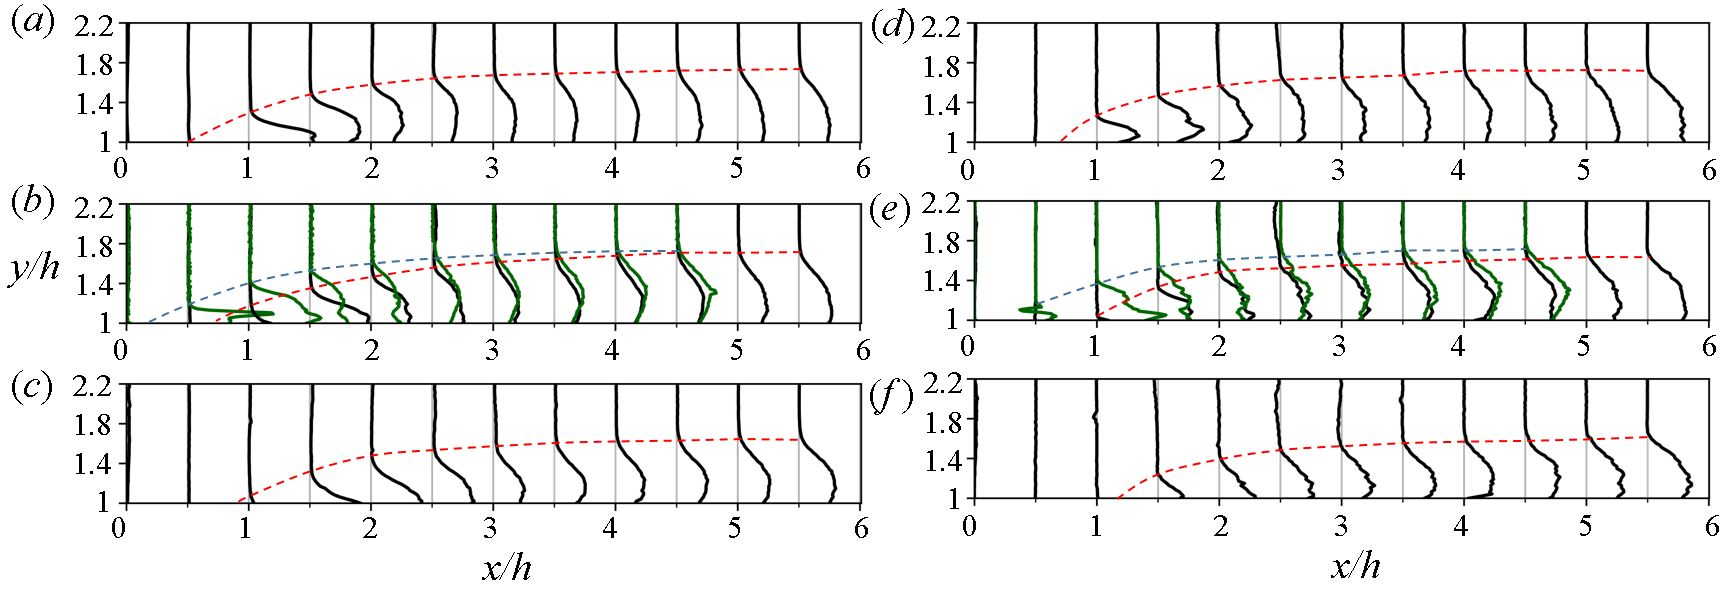
\includegraphics[width=1\textwidth]{TKE_uv_profiles}}
	\caption{TKE profiles $ \langle {u^{\prime}}^2 + {v^{\prime}}^2 \rangle/(2U_{\infty}^2)$ above the canopy with various incoming flow condition: $(a)$ $Ca = 2.3$, $(b)$ $Ca = 5.1$, $(c)$ $Ca = 9.0$. d-f) Kinematic shear stress profiles.  }
	\label{TKE_profile}
\end{figure}

\begin{figure}
	\centerline{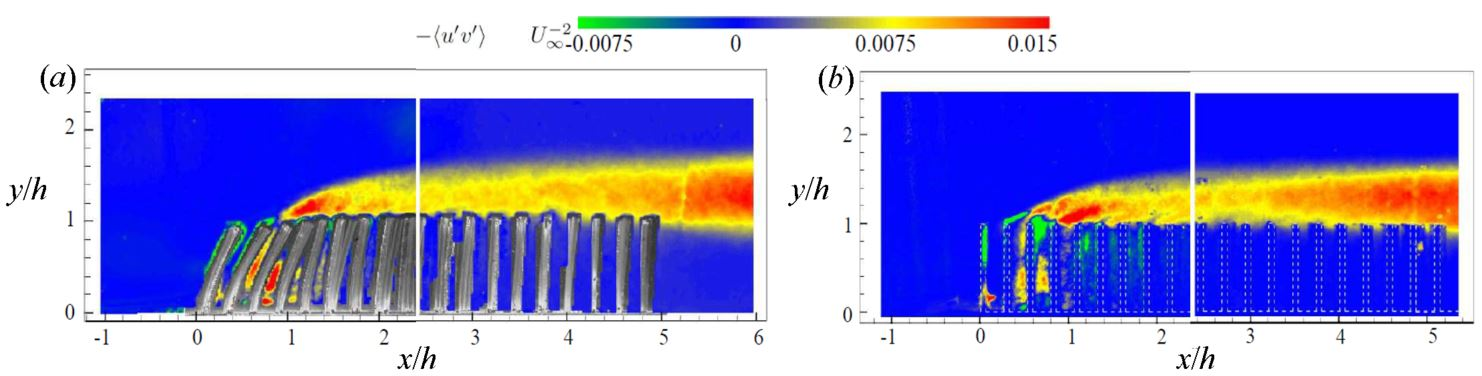
\includegraphics[width=1\textwidth]{uw}}
	\caption{Reynolds shear stress fields $-\langle u^{\prime} v^{\prime} \rangle  /{U_{\infty}}^2$ at $Re_H = 27614$. }
	\label{RSS_contour}
\end{figure}

\begin{figure}
	\centerline{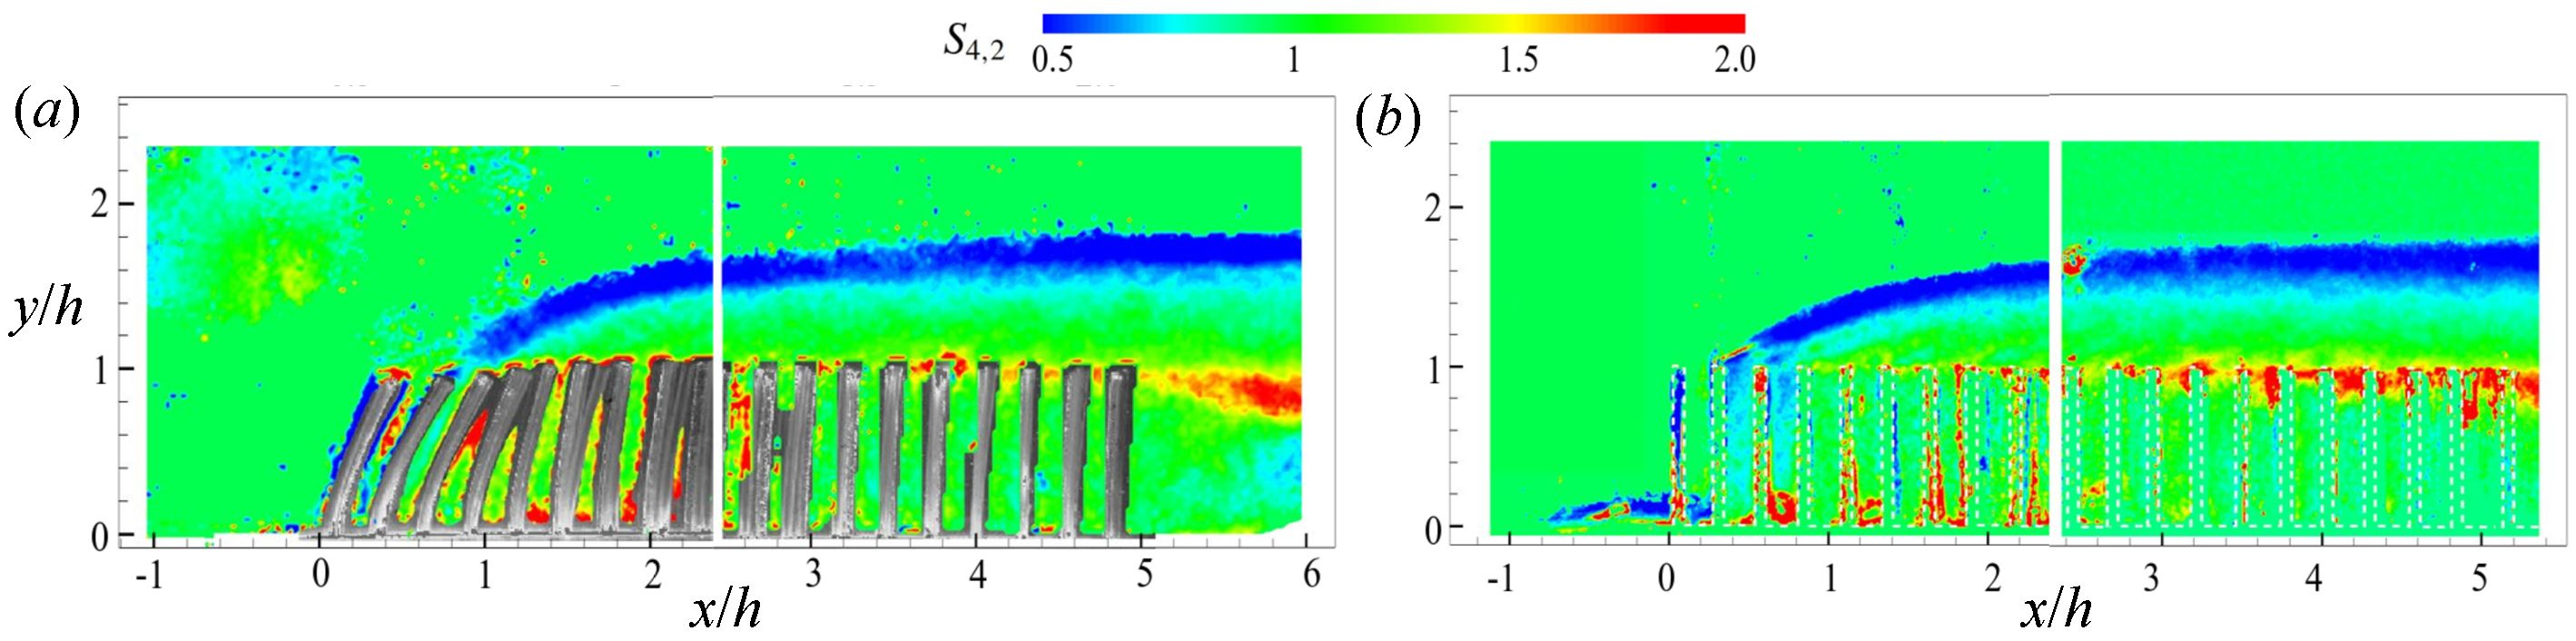
\includegraphics[width=0.95\textwidth]{Qd}}
	\caption{Quadrant of the Reynolds shear stress fields $-\langle u^{\prime} v^{\prime} \rangle  /{U_{\infty}}^2$ at $Re_H = 27614$. }
	\label{RSS_contour}
\end{figure}

\begin{figure}
	\centerline{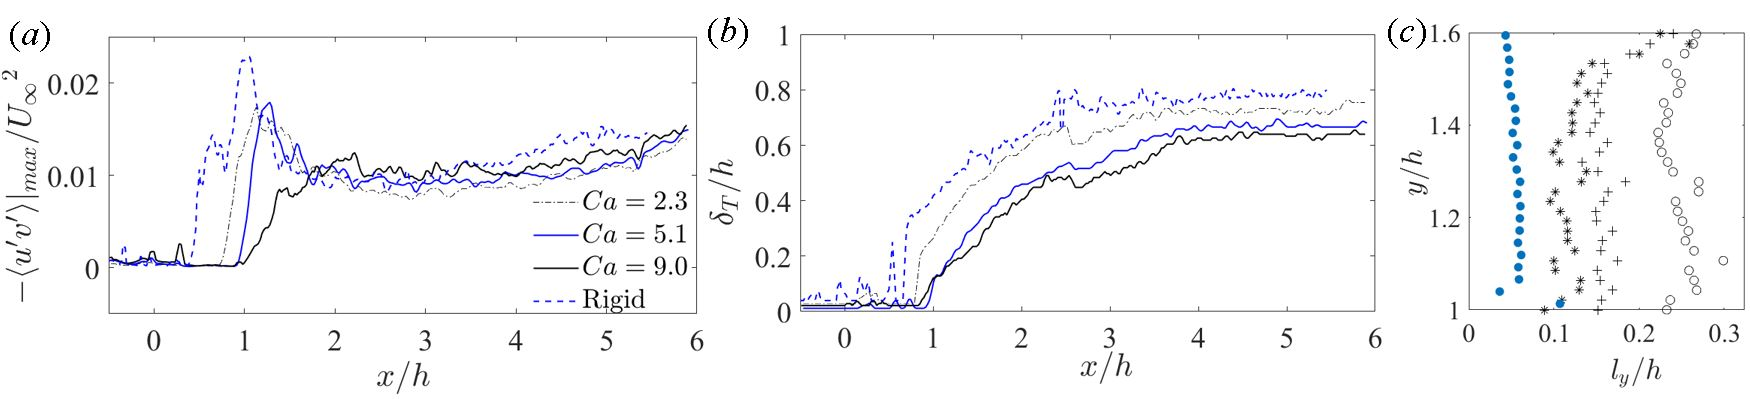
\includegraphics[width=\textwidth]{uw_d_ly}}
	\caption{RSS profiles $-\langle u^{\prime} v^{\prime} \rangle/ U_{\infty}^{2}$ above the canopy with various incoming flow condition: $(a)$ $Re_H = 18409$; $(b)$ $Re_H = 27614$; $(c)$ $Re_H = 36818$. }
	\label{RSS_profile}
\end{figure}

\begin{figure}
	\centering
		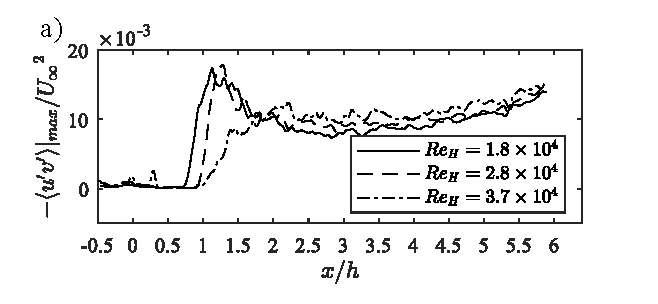
\includegraphics[width=0.49\linewidth]{rssmax}
		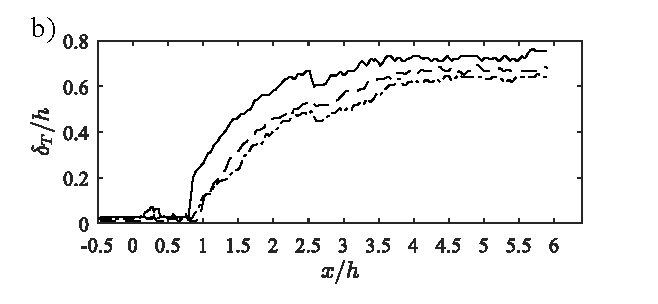
\includegraphics[width=0.49\linewidth]{thickness}
	\caption{Maximum RSS profiles $-\langle u^{\prime} v^{\prime} \rangle |_{max}/  U_{\infty}^{2}$ above the canopy with various incoming flow conditions: $(a)$ $Re_H = 18409$; $(b)$ $Re_H = 27614$; $(c)$ $Re_H = 36818$; Extension of mixing layer $\delta_T h^{-1}$ above the canopy with various incoming flow conditions: $(d)$ $Re_H = 18409$; $(e)$ $Re_H = 27614$; $(f)$ $Re_H = 36818$.}
	\label{RSSmaxthickness}
\end{figure}

 

\begin{figure}
	\centerline{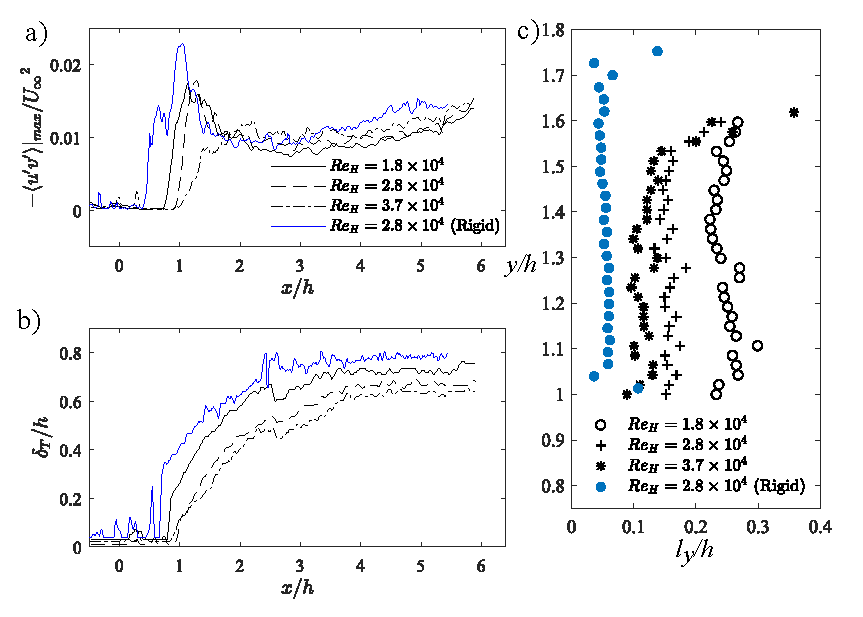
\includegraphics[width=0.8\textwidth]{MixingLength}}
	\caption{Vertical mixing length $l_y = \sqrt{-\langle u^{\prime}v^{\prime}  \rangle {\big( \frac{\partial U}{\partial y} \big)}^{-2}}$ above the canopy with various incoming flow conditions: $(a)$ $Re_H = 18409$; $(b)$ $Re_H = 27614$; $(c)$ $Re_H = 36818$.}
	\label{mixinglength}
\end{figure}


 \subsection{On the dynamics of the plate motions}

\begin{figure}
	\centerline{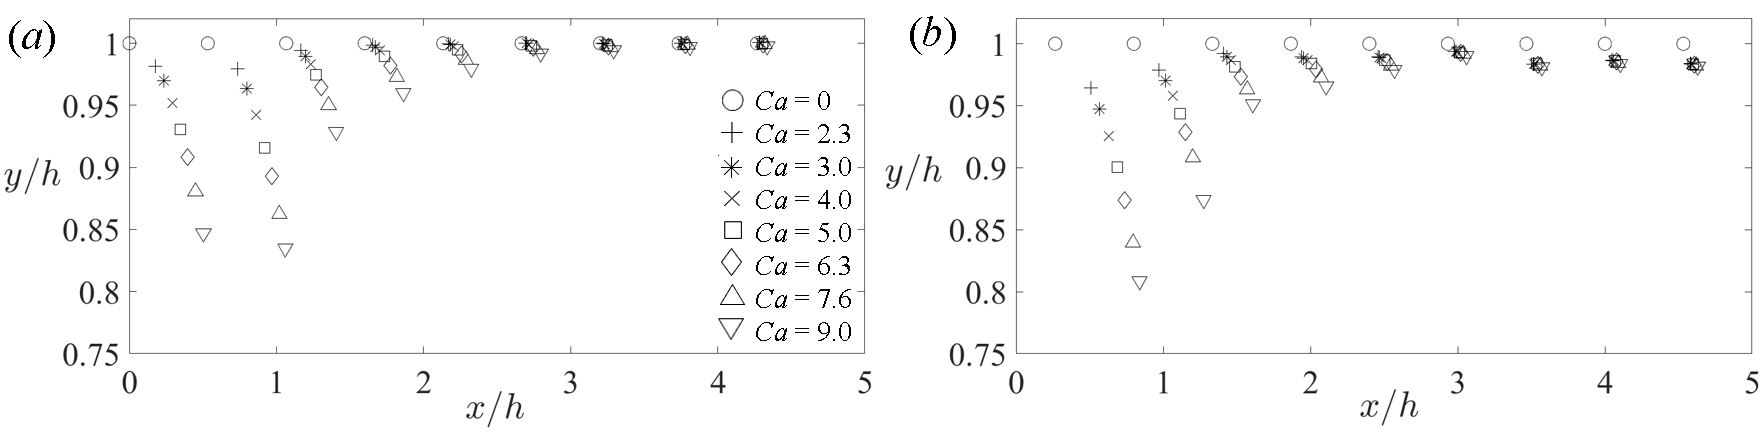
\includegraphics[width=\textwidth]{Bending}}
	\caption{Time-averaged tip position with various incoming flow velocity: No incoming flow ($\bigcirc$), $Re_H = 1.8 \times 10^4$ ($+$); $Re_H = 2.1 \times 10^4$ ($*$); $Re_H = 2.5 \times 10^4$ ($\times$); $Re_H = 2.8 \times 10^4$ ($\square$); $Re_H = 3.1 \times 10^4$ ($\Diamond$); $Re_H =3.4 \times 10^4$ ($\bigtriangleup$); $Re_H =3.7 \times 10^4$ ($\bigtriangledown$).$(a)$ central column of canopy (upper red dash line in figure \ref{canopy_model}); $(b)$  nearest column of canopy. (lower red dash line in figure \ref{canopy_model})}
	\label{average_tip}
\end{figure}




 

\begin{figure}[]
	\centerline{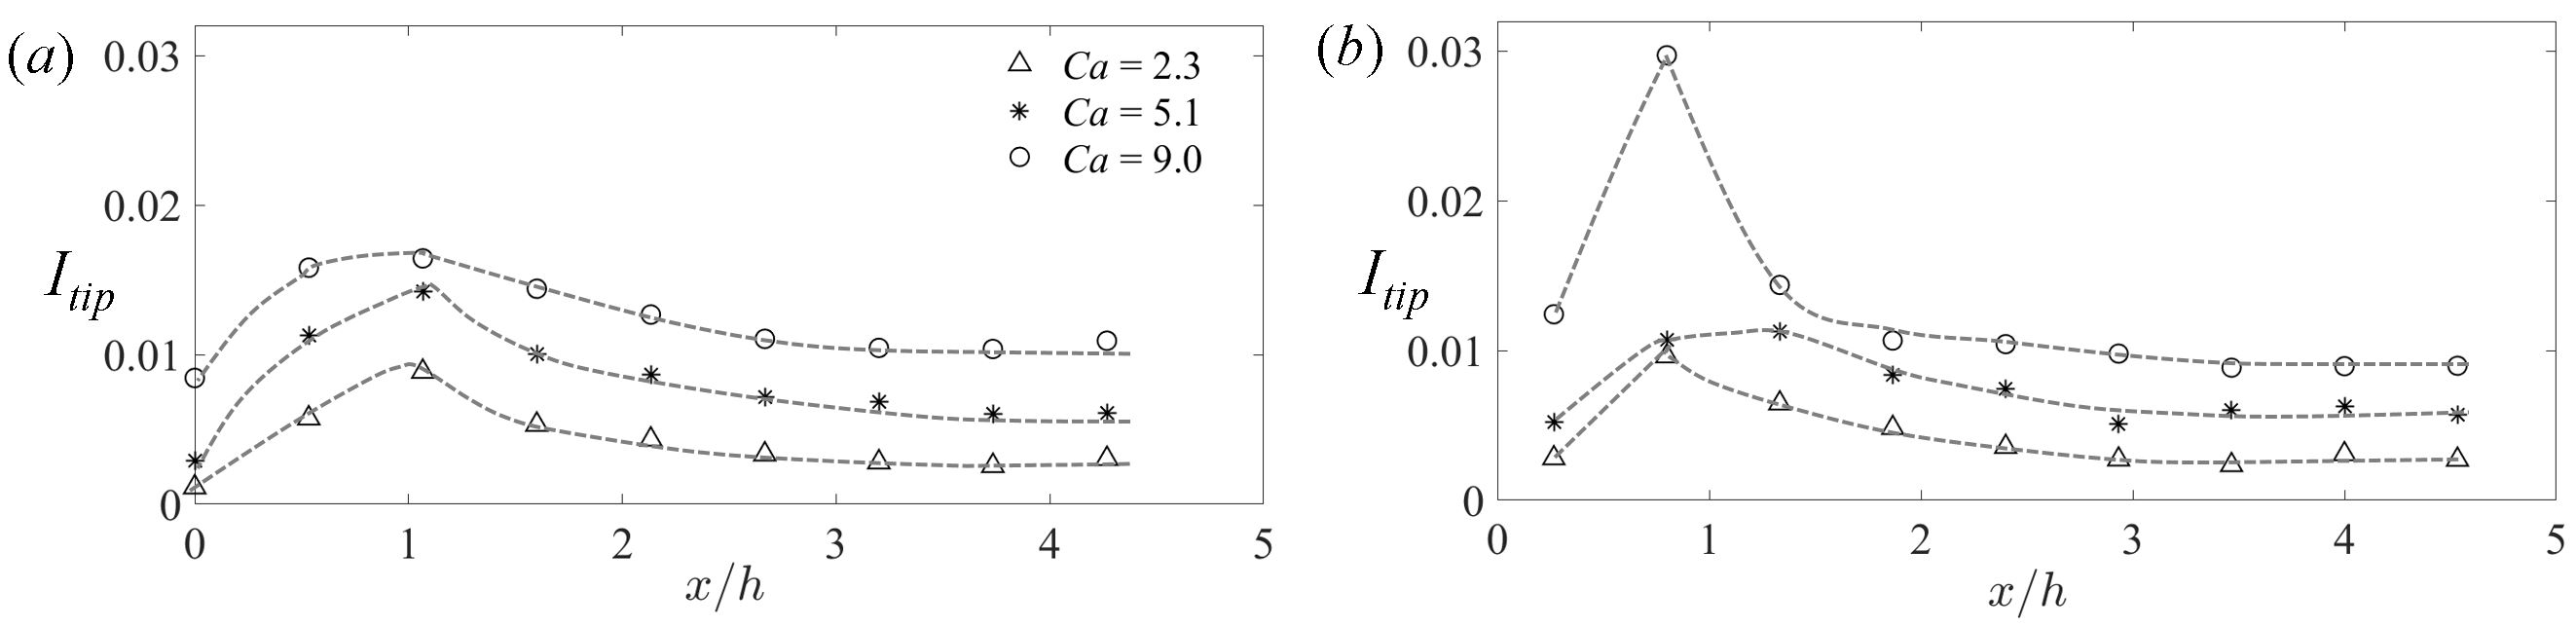
\includegraphics[width=1\textwidth]{I}}
	\caption{Displacement intensity $I_{tip} = |x(t) - X_0|$ above the canopy  with various incoming flow conditions: $Re_H = 18409$, $Re_H = 27614$, $Re_H = 36818$. And figure a is the center row(Top dashed line in figure \ref{canopy_model}), figure b is the adjacent row(Lower dashed line in figure \ref{canopy_model}). }
	\label{intensity}
\end{figure}

\begin{figure}[]
    \centering
         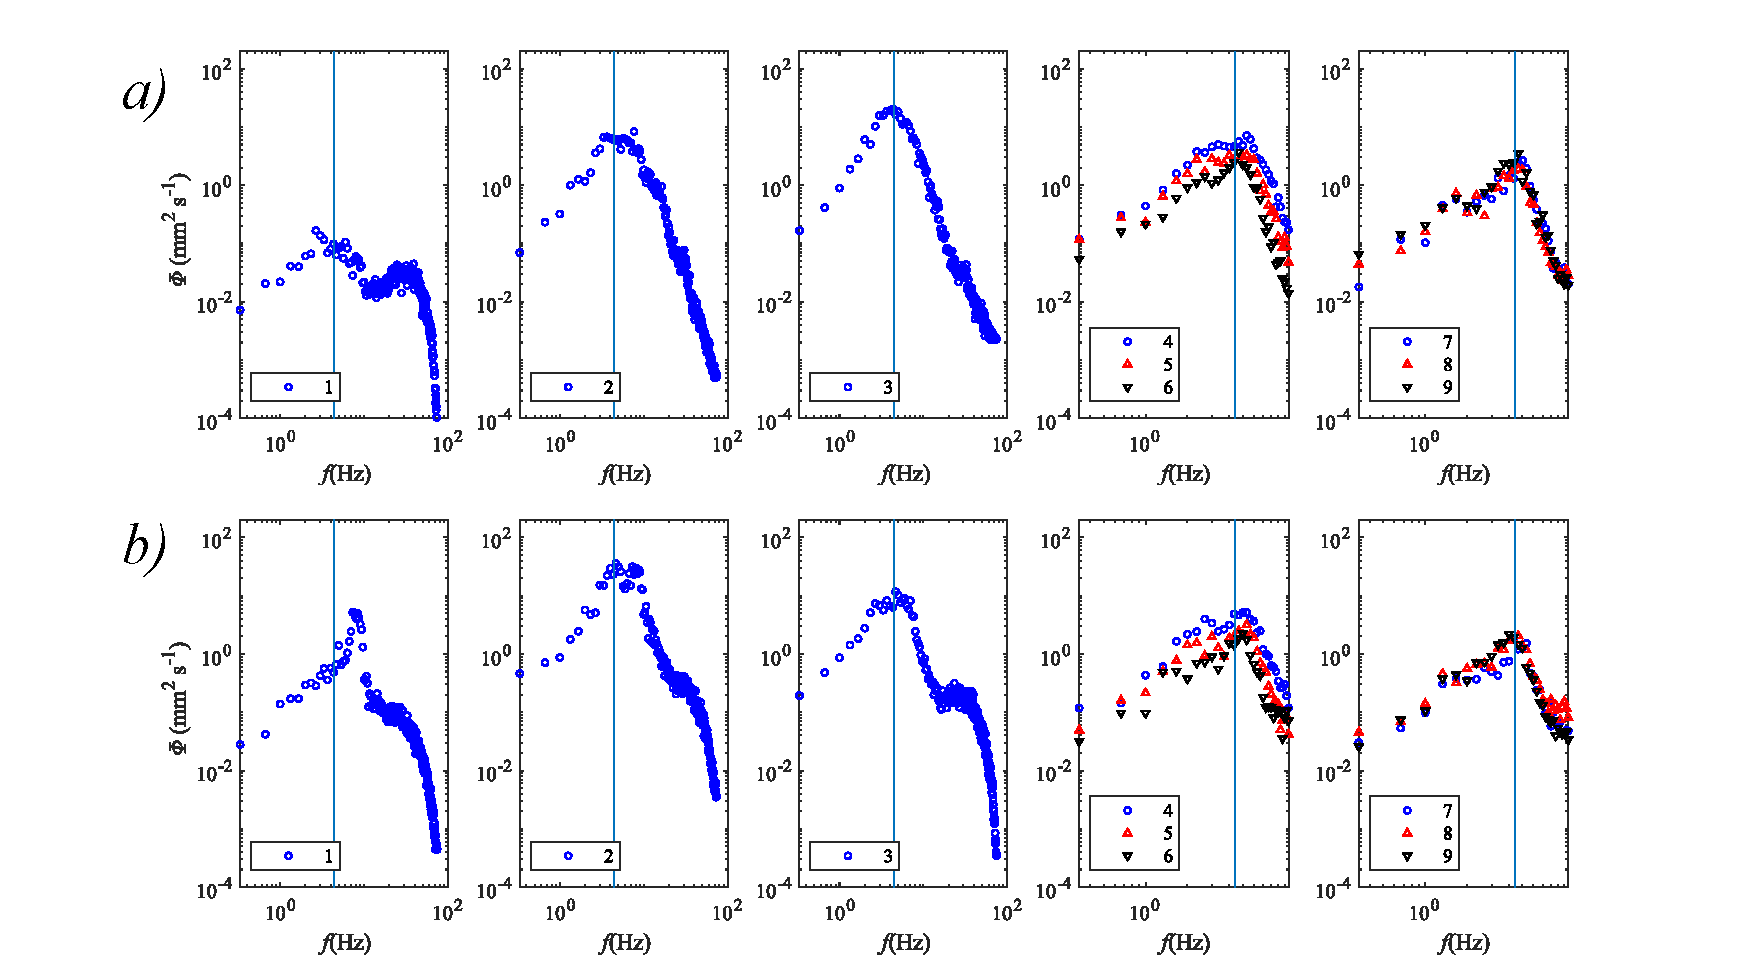
\includegraphics[width=.8\linewidth]{6hz_spectra}
        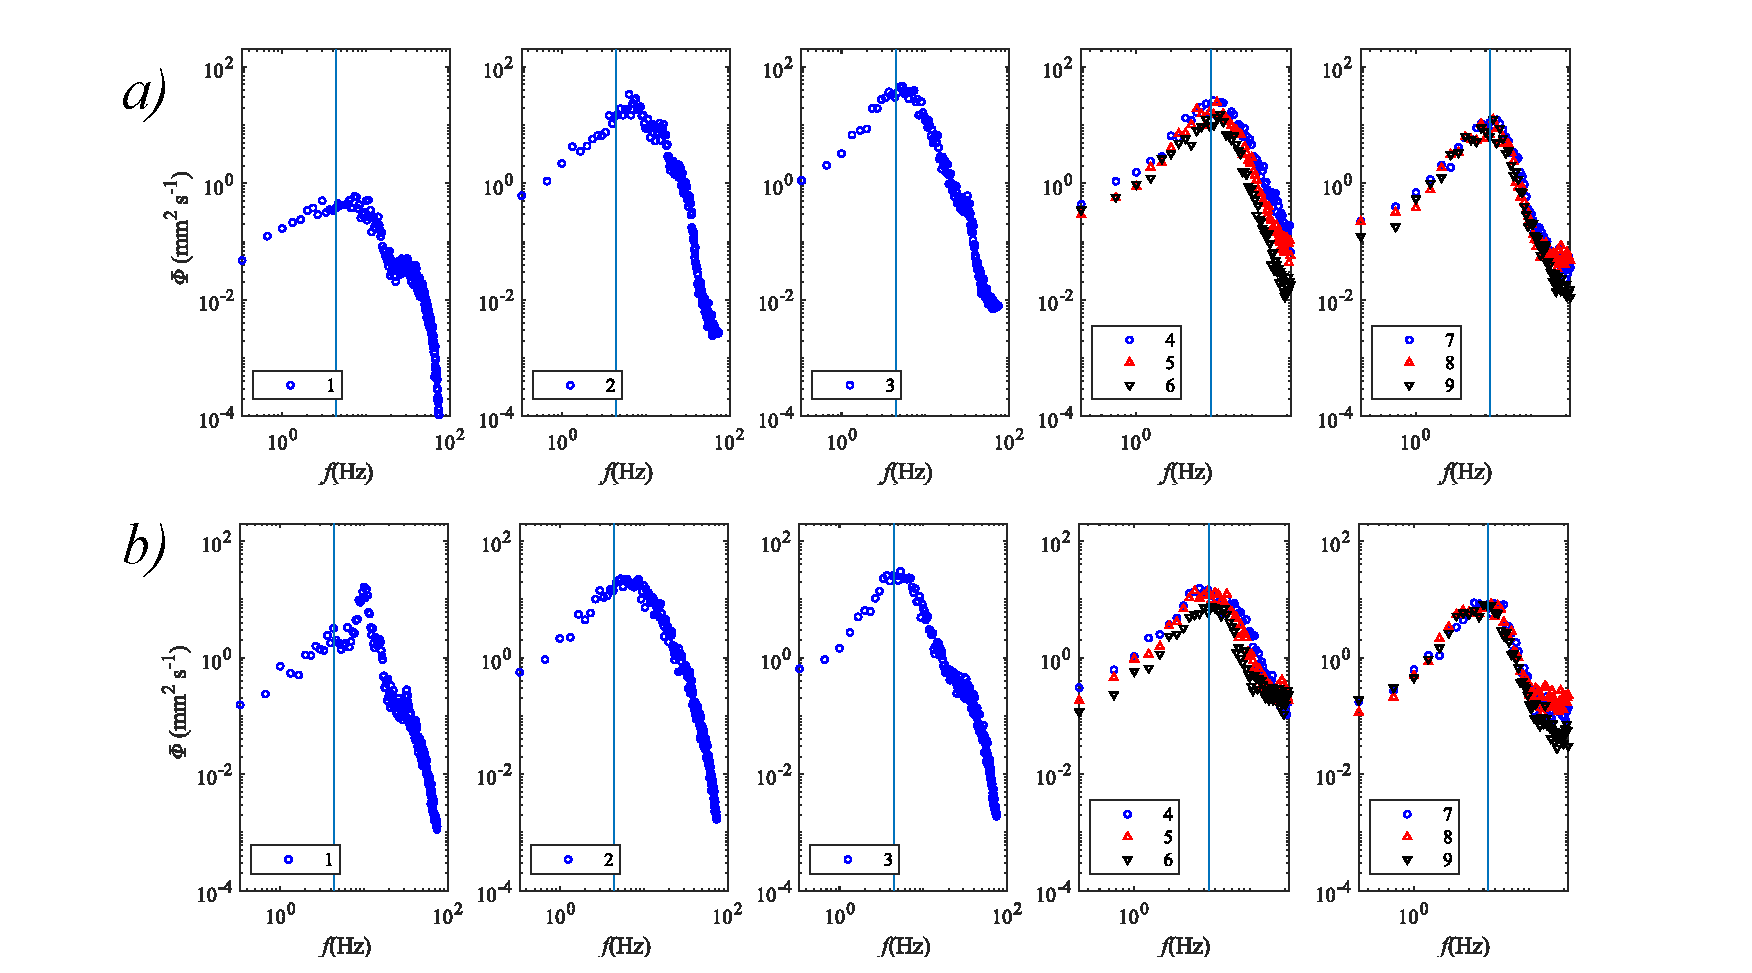
\includegraphics[width=.8\linewidth]{9hz_spectra}
        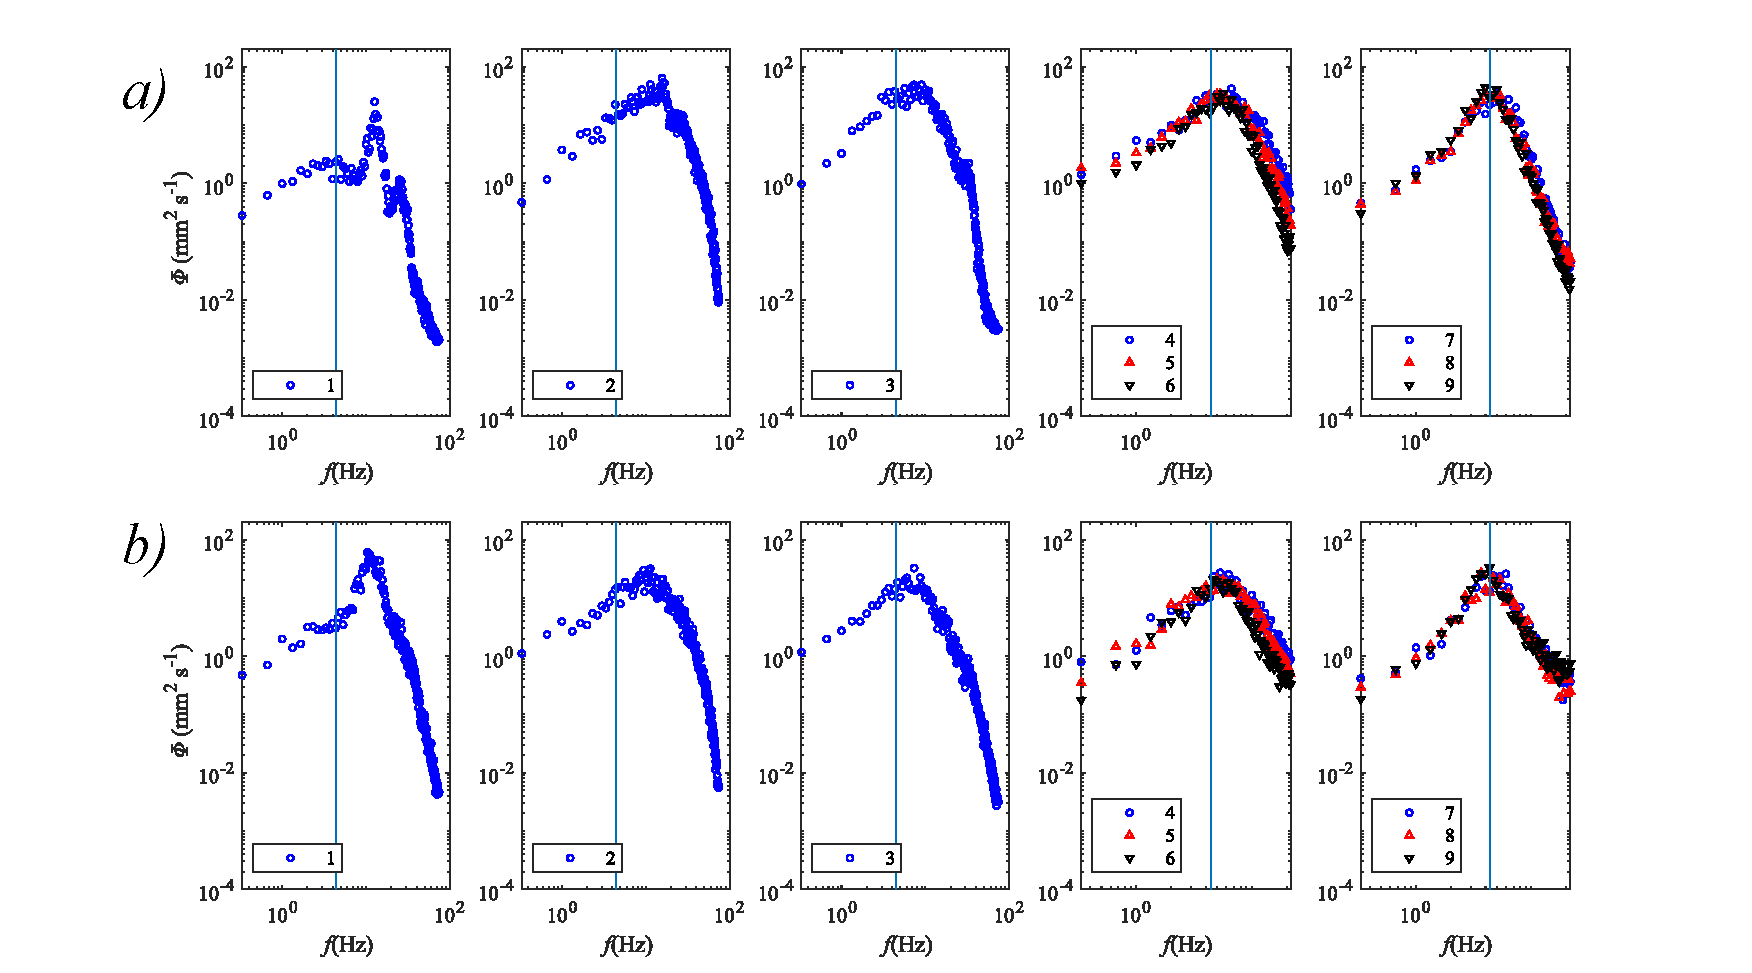
\includegraphics[width=.8\linewidth]{12hz_spectra}
    \caption{Velocity spectra for all incoming flow conditation: $(a)$ center row; $(b)$ adjacent row. The numerical legend in figure indicates the rank of canopy countered from leading edge. The vertical line is the first order natural frequency.}
    \label{spectra}
\end{figure}


\begin{figure}[]
	\centerline{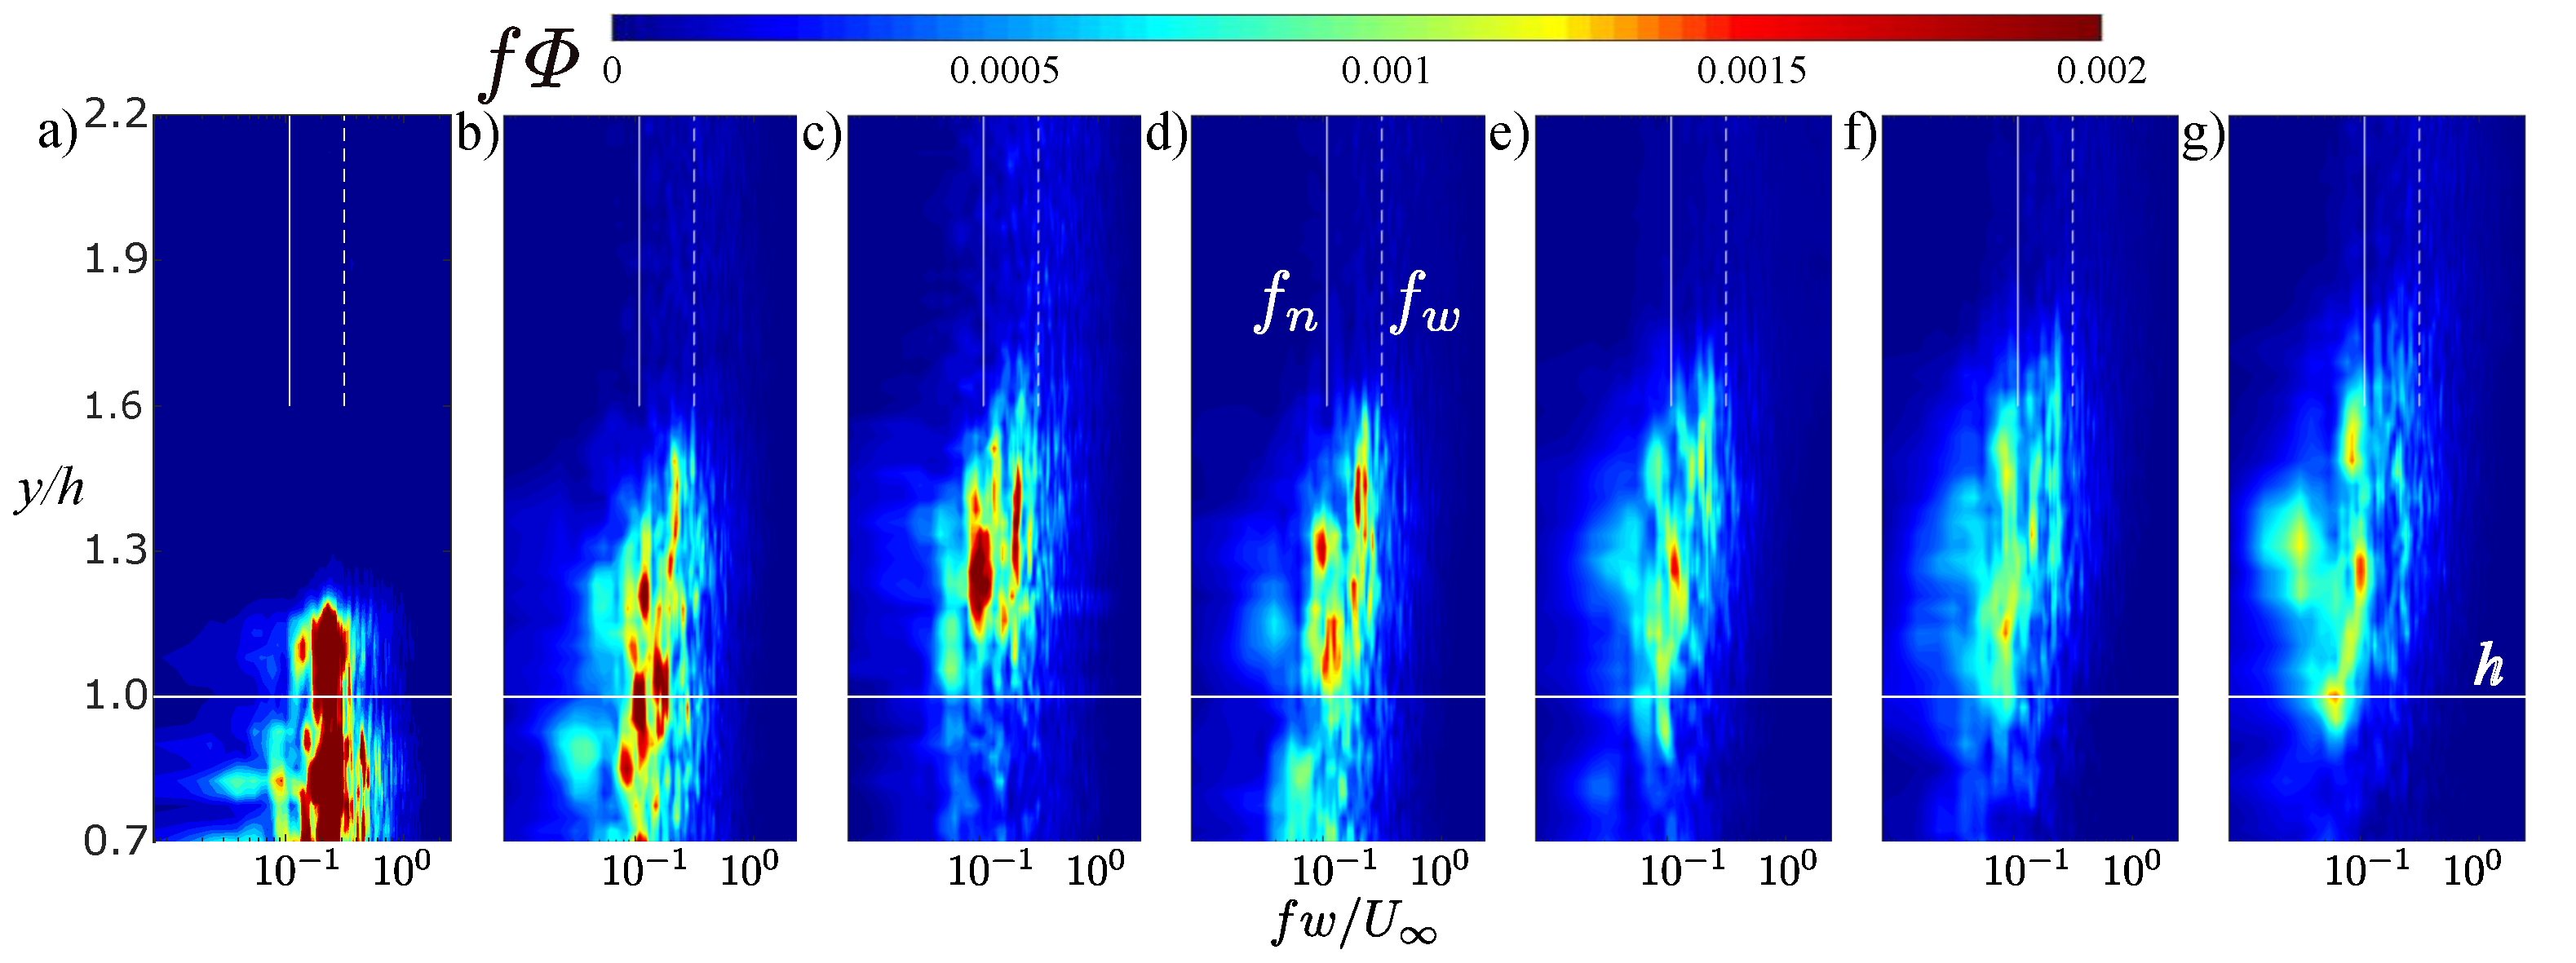
\includegraphics[width=1\textwidth]{spec_piv}}
	\caption{Velocity spectrum $\Phi * f$ contour plot at various x position with $St = f * w / U_{\infty}$. The white solid lines indicate the natural frequency of canopy and the white dash lines indicate the flow induced frequency.}
	\label{flow_spectra}
\end{figure}

\begin{figure}[]
	\centerline{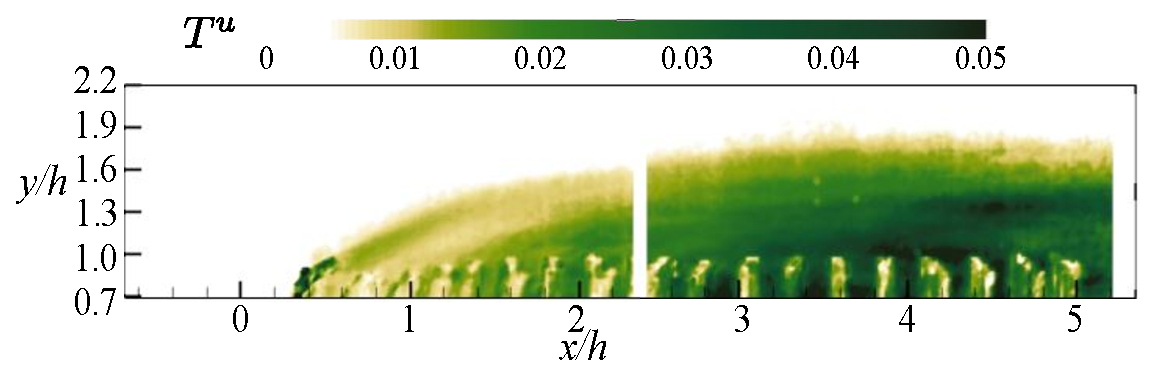
\includegraphics[width=0.7\textwidth]{auto}}
	\caption{}
	\label{auto}
\end{figure}

 


\subsection{On the equivalent local force acting on the plates}













\begin{Backmatter}

\paragraph{Acknowledgements}
We gratefully acknowledge the advice of John Smith who
commented on a version of this manuscript.

\paragraph{Funding Statement}
J.G.S gratefully acknowledges funding by an NSF CAREER
Award (Contract number NSF CTS0239080) with Dr. Michael W.
Plesniak as contract monitor.

\paragraph{Declaration of Interests}
The authors declare no conflict of interest.

\paragraph{Author Contributions}
R.B. and J.G.S. created the research plan, designed
experiments, and formulated analytical problem. R.B. led
model solution and performed all experiments. R.B. and
J.G.S. wrote the manuscript.

\paragraph{Data Availability Statement}
Raw data are available from the corresponding author
(J.G.S.).

\paragraph{Ethical Standards}
The research meets all ethical guidelines, including
adherence to the legal requirements of the study country.

\paragraph{Supplementary Material}
Methods section and Supplementary information are available
at \url{https://doi.org/10.1017/flo.2021.1}.




\end{Backmatter}

\end{document}
